\documentclass{beamer}
\usetheme{Madrid}

\usepackage[utf8]{inputenc}
%\usepackage{beamerthemeshadow}
%\usepackage{stmaryrd} % Needed for \bigsqcap
%\usepackage{algorithm}
%\usepackage{algpseudocode}


\definecolor{Green}{rgb}{0.506, 0.727, 0.396} % (primary)

\usecolortheme[named=Green]{structure}

\newcommand\owlIndent{\hspace{4mm}}
\newcommand\setspacing{\hspace{2pt}}

\renewcommand{\arraystretch}{1.2} % Vertical spacing of rows in table



\begin{document}
\title{SubClassOf vs EquivalentTo}
\author{Henriette Harmse}
\date{}

\frame{\titlepage}
%\AtBeginSection[]
%{
%  \begin{frame}<beamer>
%    \frametitle{Outline}
%    \tableofcontents[]
%  \end{frame}
%}

\frame{\frametitle{Prerequisites}
	Before doing this tutorial you need to have the following knowledge:	
	\begin{enumerate}
		\item Building blocks of OWL and Description Logics
	\end{enumerate}
}

\frame{\frametitle{The semantics of \texttt{SubClassOf}}
	\begin{block}{Syntax}
		\begin{table} 
			\begin{center} 
				\begin{small}
					\begin{tabular}{|c|c|c|} 
						\hline					
							\textbf{OWL}&\textbf{DL}&\textbf{Semantics}\\
						\hline 
							\begin{minipage}{4cm}
								$\begin{aligned}
									&\texttt{Class: C}\\
									&\owlIndent\texttt{SubClassOf: D}\\
									&\texttt{Class: D}
								\end{aligned}$
							\end{minipage}				
							& 
							\begin{minipage}{2cm}
								$\begin{aligned}
									C \sqsubseteq D
								\end{aligned}$
							\end{minipage}
							&
							\begin{minipage}{4cm}
								%trim option's parameter order: left bottom right top
								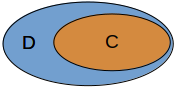
\includegraphics[trim = 0mm 0mm 0mm 0mm, clip, scale=0.4]{./images/CsubClassOfD.png}
							\end{minipage}										
							\\
						\hline						 				  
					\end{tabular}
				\end{small}
			\end{center}
		\end{table}
	\end{block}
	\begin{block}{Semantics}
	The set $C$ is a subset of the set $D$. This means every individual of $C$ is necessarily an individual of $D$, but not every individual of $D$ is necessarily an individual of $C$.
	\end{block}
}

%\subsection{Example and guidance}
\frame{\frametitle{The semantics of \texttt{SubClassOf}}
	\begin{block}{Example}
		\begin{table} 
			\begin{center} 
				\begin{small}
					\begin{tabular}{|c|c|c|} 
						\hline					
						\textbf{OWL}&\textbf{DL}&\textbf{Semantics}\\
						\hline 
						\begin{minipage}{4cm}
							$\begin{aligned}
								&\texttt{Class: Dog}\\
								&\owlIndent\texttt{SubClassOf: Pet}\\
								&\texttt{Class: Pet}
							\end{aligned}$
						\end{minipage}				
						& 
						\begin{minipage}{2cm}
							$\begin{aligned}
								Dog \sqsubseteq Pet
							\end{aligned}$
						\end{minipage}
						&
						\begin{minipage}{4cm}
							%trim option's parameter order: left bottom right top
							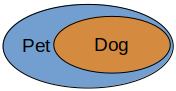
\includegraphics[trim = 0mm 0mm 0mm 0mm, clip, scale=0.4]{./images/CsubClassOfDExample.png}
						\end{minipage}										
						\\
						\hline						 				  
					\end{tabular}
				\end{small}
			\end{center}
		\end{table}
	\end{block}
	\begin{block}{Guidance - When not to use}
	\begin{table} 
		\begin{center} 
			\begin{small}
				\begin{tabular}{|c|c|} 
					\hline					
					\textbf{When not use}&\textbf{Venn diagram}\\
					\hline 
					\begin{minipage}{6cm}
						When there is an individual of $C$ that is not an individual of $D$.
					\end{minipage}									
					& 
					\begin{minipage}{4cm}
						%trim option's parameter order: left bottom right top
						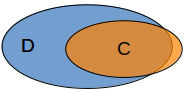
\includegraphics[trim = 0mm 1mm 0mm 1mm, clip, scale=0.4]{./images/SubClassOfWhenNotToUse.png}
					\end{minipage}										
					\\
					\hline 
					\begin{minipage}{6cm}
						When every individual of $D$ is also an individual of $C$, then prefer using \texttt{EquivalentTo}.
					\end{minipage}									
					& 
					\begin{minipage}{4cm}
						%trim option's parameter order: left bottom right top
						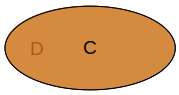
\includegraphics[trim = 0mm 1mm 0mm 1mm, clip, scale=0.4]{./images/EquivalentTo.png}
					\end{minipage}										
					\\					
					\hline						 				  
				\end{tabular}
			\end{small}
		\end{center}
	\end{table}
	\end{block}
}

%\section{The semantics of \texttt{EquivalentTo}}
\frame{\frametitle{The semantics of \texttt{EquivalentTo}}
	\begin{block}{Syntax}
	\begin{table} 
		\begin{center} 
			\begin{small}
				\begin{tabular}{|c|c|c|} 
					\hline					
					\textbf{OWL}&\textbf{DL}&\textbf{Semantics}\\
					\hline 
					\begin{minipage}{5.25cm}
						$\begin{aligned}
							&\texttt{Class: C}\\
							&\owlIndent\texttt{EquivalentTo: D}\\
							&\texttt{Class: D}
						\end{aligned}$
						\smallskip\\
						\text{which can be seen as shorthand for:}
						\smallskip
						$\begin{aligned}
							&\texttt{Class: C}\\
							&\owlIndent\texttt{SubClassOf: D}\\
							&\texttt{Class: D} \\
							&\owlIndent\texttt{SubClassOf: C}\\
						\end{aligned}$					
					\end{minipage}				
					& 
					\begin{minipage}{2cm}
						$\begin{aligned}
							C \equiv D
						\end{aligned}$\\
					which can be seen as shorthand for
					\smallskip\\
						$\begin{aligned}
							C \sqsubseteq D \\
							D \sqsubseteq C
						\end{aligned}$					
					\end{minipage}
					&
					\begin{minipage}{2.75cm}
						%trim option's parameter order: left bottom right top
						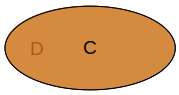
\includegraphics[trim = 0mm 0mm 0mm 0mm, clip, scale=0.4]{./images/EquivalentTo.png}
					\end{minipage}										
					\\
					\hline						 				  
				\end{tabular}
			\end{small}
		\end{center}
	\end{table}
\end{block}
\begin{block}{Semantics}
	Every individual of $C$ is an individual of $D$, \textbf{and} every individual of $D$ is an individual of $C$.
\end{block}
}




\frame{\frametitle{The semantics of \texttt{EquivalentTo}}
	\begin{block}{Example}
		\begin{table} 
			\begin{center} 
				\begin{small}
					\begin{tabular}{|c|c|c|} 
						\hline					
						\textbf{OWL}&\textbf{DL}&\textbf{Semantics}\\
						\hline 
						\begin{minipage}{4cm}
							$\begin{aligned}
								&\texttt{Class: Person}\\
								&\owlIndent\texttt{EquivalentTo: Human}\\
								&\texttt{Class: Human}
							\end{aligned}$
						\end{minipage}				
						& 
						\begin{minipage}{3cm}
							$\begin{aligned}
								Person \sqsubseteq Human
							\end{aligned}$
						\end{minipage}
						&
						\begin{minipage}{3cm}
							%trim option's parameter order: left bottom right top
							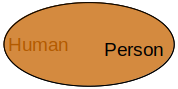
\includegraphics[trim = 0mm 0mm 0mm 0mm, clip, scale=0.4]{./images/EquivalentToExample.png}
						\end{minipage}										
						\\
						\hline						 				  
					\end{tabular}
				\end{small}
			\end{center}
		\end{table}
	\end{block}
	\begin{block}{Guidance - When not to use}
		\begin{table} 
			\begin{center} 
				\begin{small}
					\begin{tabular}{|c|c|} 
						\hline					
						\textbf{When not use}&\textbf{Venn diagram}\\
						\hline 
						\begin{minipage}{7.5cm}
							When there is an individual of $C$ that is not in $D$.
						\end{minipage}									
						& 
						\begin{minipage}{3cm}
							%trim option's parameter order: left bottom right top
							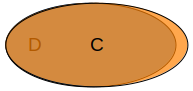
\includegraphics[trim = 0mm 0mm 0mm 0mm, clip, scale=0.4]{./images/IndividualOfCnotInD.png}
						\end{minipage}										
						\\
						\hline 
						\begin{minipage}{7.5cm}
							When there is an individual of $D$ that is not in $C$.
						\end{minipage}									
						& 
						\begin{minipage}{3cm}
							%trim option's parameter order: left bottom right top
							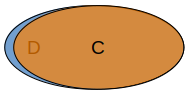
\includegraphics[trim = 0mm 1mm 0mm 1mm, clip, scale=0.4]{./images/IndividualOfDnotInC.png}
						\end{minipage}										
						\\					
						\hline						 				  
					\end{tabular}
				\end{small}
			\end{center}
		\end{table}
	\end{block}
}


\end{document}
